\begin{frame}[t,label=electroweak]
 \frametitle{Electroweak Interaction}
 \begin{columns}
  \begin{column}{0.99\textwidth}
   \begin{block}{Glashow--Weinberg--Salam theory of weak interaction}
    \begin{itemize}
     \item Gauge symmetry: $SU(2)_L \times U(1)_Y$
     \item Gauge couplings: $g$ for $SU(2)_L$, $g'$ for $U(1)_Y$
     \item \alert{Left-handed leptons} in doublets, \alert{right-handed} in singlets
     \item \alert{Fundamental symmetry of left and right helicity broken}
    \end{itemize}
   \end{block}
  \end{column}
  \begin{column}{0.01\textwidth}
  \end{column}
 \end{columns}
\only<1>{
 \begin{columns}
  \begin{column}{0.65\textwidth}
   \begin{block}{Parity symmetry is violated}
    \begin{itemize}
     \item \alert{Weak interaction violates parity}
     \item Electromagnetic interaction still satisfies parity
     \item Use parity-violation to measure electroweak parameters
    \end{itemize}
   \end{block}
  \end{column}
  \begin{column}{0.35\textwidth}
   \pgfimage[width=\textwidth]{images/qweak/Parity_Violation_Cartoon}
  \end{column}
 \end{columns}
}
\only<2>{
 \begin{columns}
  \begin{column}{0.99\textwidth}
   \begin{block}{Electroweak symmetry breaking: $B_\mu, W^i_\mu \to A_\mu, Z^0_\mu, W^\pm_\mu$}
    \small
    \begin{equation*}
     \alert{\sin^2 \theta_W} = \frac{g'^2}{g^2 + g'^2} = 0.23122 \pm 0.00015 \approx \frac{1}{4} \quad (\hbox{at}~M_Z)
    \end{equation*}
    \begin{eqnarray*}
     A_\mu & = & \alert{\cos \theta_W} \cdot B_\mu + \alert{\sin \theta_W} \cdot W^3_\mu \qquad (\hbox{massless photon field}) \\
     Z^0_\mu & = & - \alert{\sin \theta_W} \cdot B_\mu + \alert{\cos \theta_W} \cdot W^3_\mu \quad (M_W \approx 80.4\,\hbox{GeV}, M_Z \approx 91.2\,\hbox{GeV})
    \end{eqnarray*}
   \end{block}
  \end{column}
  \begin{column}{0.01\textwidth}
  \end{column}
 \end{columns}
}
\only<3>{
 \begin{columns}
  \column{0.7\textwidth}
   \begin{block}{Parity-violation neutral current}
    \small
    \begin{eqnarray*}
     \mathcal{L}^{EW}_{PV} = -\frac{G_F}{\sqrt{2}} & \left[ g^e_A \left( \red{\bar{e} \gamma_\mu \gamma_5 e} \right) \cdot \sum_i g^q_V \left( \blue{\bar{q} \gamma^\mu q} \right) \right. \\
     + & \left. g^e_V \left( \red{\bar{e} \gamma_\mu e} \right) \cdot \sum_i g^q_A \left( \blue{\bar{q} \gamma^\mu \gamma_5 q} \right) \right]
    \end{eqnarray*}
   \end{block}
  \column{0.3\textwidth}
   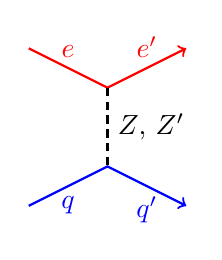
\begin{tikzpicture}[thick]
    % Electron
    \draw[red,->] (0,2.5) -- node[above]{$e$} (1,2) -- node[above]{$e'$} (2,2.5);
    % Z boson
    \draw[densely dashed] (1,2) -- node[right]{$Z$, $Z'$} (1,1);
    % Quark
    \draw[blue,->] (0,0.5) -- node[below]{$q$} (1,1) -- node[below]{$q'$} (2,0.5);
   \end{tikzpicture}
 \end{columns}
}
\end{frame}
